\documentclass[11pt,a4paper]{article}
\usepackage{lac2017}
\usepackage{graphicx}
\usepackage{listings}
\sloppy
\newenvironment{contentsmall}{\small}

\title{Using Physical Modeling in Faust}
% RM: TODO mmmh

%see lac2015.sty for how to format multiple authors!
\author
{P.-A. GRUMIAUX${}^1$, R. MICHON${}^2$, 
E. GALLEGO ARIAS${}^1$, P. JOUVELOT${}^1$
\\ ${}^1$MINES ParisTech, PSL Research University, France  
\\ ${}^2$ CCRMA, Stanford University, USA
}

\newcommand{\f}{\textsc{Faust}}

\begin{document}
\maketitle


\begin{abstract}
  \begin{contentsmall}
    % RM: might have to be a bit more direct here TODO
This paper presents a use case for a library written in the \f{} language providing tools to synthesize sound using physical modeling. The first section gives an overview of Faust and physical modeling theory. In the second section, we focus on the implementation of the library and how it can be used. The last section describes two python scripts % TODO.
\end{contentsmall}
\end{abstract}

\keywords{
\begin{contentsmall}
Physical modeling synthesis, Faust language, digital signal processing
\end{contentsmall}
}

\section{Introduction}

Sound synthesis is an active subject of research and many programming languages have been designed and used for that purpose. Physical modeling synthesis % RM: we need a reference here
can be used to reproduce the sound of real instruments. This synthesis technique has evolved during the last twenty years of the $20^{th}$ century and was developed with the programming languages of that period. % TODO ok review the whole sentence here

\f{} % we need a reference here
is a functional programming language for real-time signal processing (DSP) and synthesis. \f{} targets high-performance DSP applications and audio plug-ins for a variety of platforms and standards. \f{} has been used in the past \cite{TODO:faustSTK} to implement physical models of musical instruments. In this paper, we present a new library to implement physical models in a modular way. It provides both low-level and high-level elements (bore, string, bridge, bow, hammer, etc.) to be used to create models of existing and novel instruments.

% TODO review that too
The first section of this paper provides a quick tour of some elements of physical modeling synthesis. The second section quickly explains how the Faust language is used to write sound processors. In the third section, we introduce the beginning of the physical modeling library in Faust with basic elements.  In the last section, we present two python scripts that provide a way to create a vibration model of an object.

\section{Physical Modeling Synthesis}

Physical modeling synthesis aims at describing real world phenomena in music instrument sounds using physical models.\cite{pasp}

\subsection{Principle}

This kind of synthesis refers to a set of methods that generate the waveform of a sound based on a mathematical model. This model is characterised by specific parameters of the instrument (size, way of excitation, material, etc.).

\subsection{Delay line}

A delay line is an elementary element modeling the acoustic propagation of sound. It inserts a time delay between its input and output as shown, in Figure \ref{fig:delayline}.

\begin{figure}[h]
	\centering
	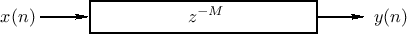
\includegraphics[scale=0.5]{pictures/delayline.png}
	\caption{An M-sample delay line}
	\label{fig:delayline}
\end{figure}

\subsection{Digital Waveguide}

A digital waveguide is defined as a bidirectional delay line (see Figure \ref{fig:waveguide}) representing two traveling waves in opposite directions. Such system is useful for modeling one-dimensional acoustic systems (strings or wind instruments).

\begin{figure}
	\centering
	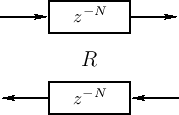
\includegraphics[scale=0.5]{pictures/waveguide.png}
	\caption{A $N$-sample-long digital waveguide}
	\label{fig:waveguide}
\end{figure}

The excitation of this type of system is specified by providing an input to both delay lines (for example, a Dirac impulse). Output are handled by adding up both signals. Such a model can be used to describe an ideal string.

\subsection{Terminations}

The last element to take into account to describe one-dimensional instruments is the ends of the system. At those terminations, the string does not move and the wave is reflected.

\begin{figure}
	\centering
	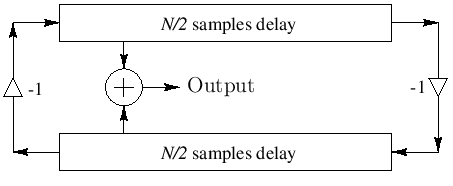
\includegraphics[scale=0.5]{pictures/terminations.png}
	\caption{Rigidly terminated string}
	\label{fig:terminations}
\end{figure}

\section{The Faust Language}

% TODO: may be move the reference somewhere else
\f{} (Functional Audio Stream) is a functional programming \cite{quickref} language designed for real-time signal processing and synthesis. It provides an adequate notation to describe signal processors and thus to quickly develop audio programs, along with block-diagram algebra.

\subsection{Syntax}

A Faust program contains a ``main'' function called \texttt{process} that consists in a signal processor.
Signal processors take input signals and give output signals, as in the identity signal processor defined by \texttt{process(x) = x;}. Common operators are usable in Faust (\texttt{+, -, *, /, mod}). The identity function can also be specified with the \texttt{\_} operator: \texttt{process = \_;}.

Block diagram compositions can be handled with common operations such as parallel composition \texttt{,}, sequential composition \texttt{:}, split composition \texttt{<:}, merge composition \texttt{:>} and the recursive composition \texttt{\~}. The \texttt{\~} operator stands for recursive composition, as in the simple counter defined by \texttt{process = + \~ \_;}. If x is the input, that block features the equation $y(n) = x(n) + y(n-1)$ (see Figure \ref{fig:recursive}).

In these compositions, the numbers of input and output signals have to be matched properly to insure proper compatibility.
\begin{figure}[h]
	\centering
	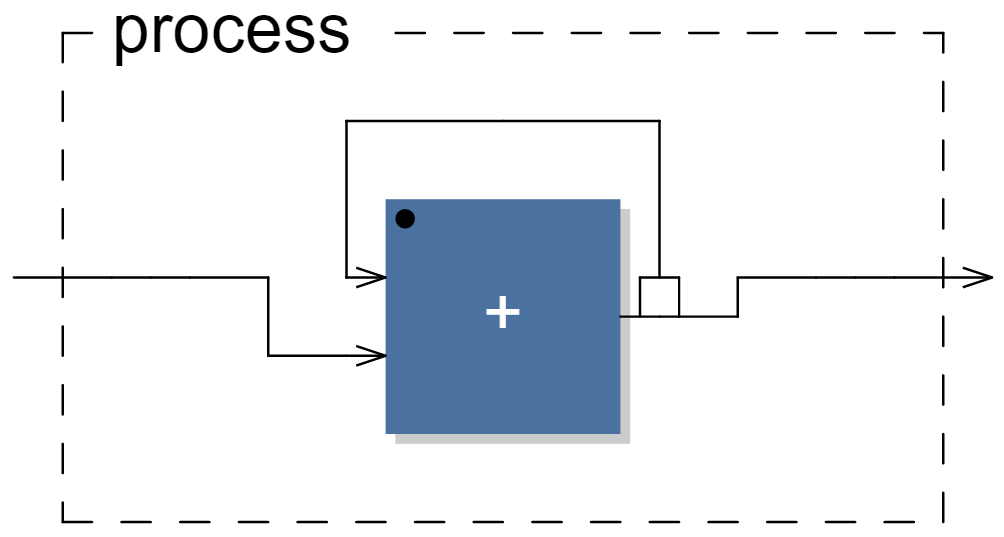
\includegraphics[scale=0.2]{pictures/recursive.png}
	\caption{Block diagram for \texttt{process = + \~ \_}}
	\label{fig:recursive}
\end{figure}

\subsection*{Diagram generation}
Block diagrams are very easy to generate using a shell command such as \texttt{faust -svg myprocessor.dsp}. This tool shows the power of Faust, which enables a musician to quickly build sound effects or instruments.

\subsection*{Libraries}
As most of programming languages, Faust comes with the possibility to import libraries, which are \texttt{.lib} files, using commands such as \texttt{import("math.lib");}. As useful libraries, we can mention \texttt{math.lib} (common math operations) and more signal-processing-oriented libraries such as \texttt{music.lib} (spatialisation, envelops, delays, etc.) and \texttt{filter.lib} (digital filters) \cite{filters}.


\section{\texttt{pm.lib}, a physical modeling library }

The Faust language as it is specified for now allows to generate only one-directional diagram blocks, from left (inputs) to right (outputs); so a bidirectional delay line as presented in Figure~\ref{fig:waveguide} cannot be implemented. 

That issue has been circumvented in the \texttt{pm.lib} library with a \texttt{chain} functions that takes both inputs to the left (plus one extra input) and gives both outputs to the right (plus one extra output to mix both signals), as shown in Diagram~\ref{fig:chain}. One main drawback of this approach is that it adds a one-sample delay to the signal.

\begin{figure}[h]
	\centering
	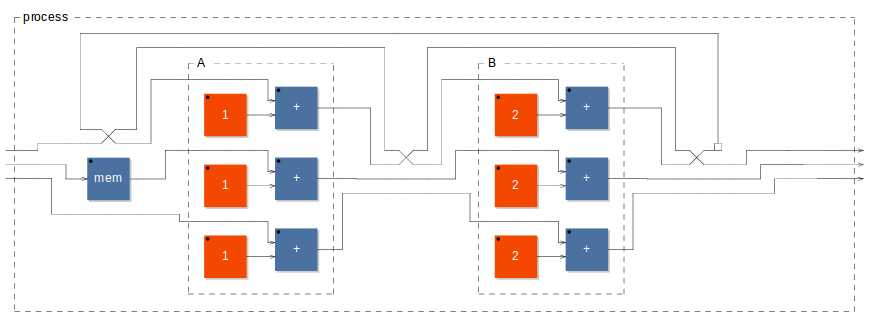
\includegraphics[scale=0.3]{pictures/chain.png}
	\caption{\texttt{chain(A:B)}, with \texttt{A=+1,+1,+1} and \texttt{B=+2,+2,+2}}
	\label{fig:chain}
\end{figure}

 The \texttt{chain} function can be more easily seen as adding up bidirectional blocks one after another, as in Figure~ \ref{fig:chainrepresentation}.

\begin{figure}[h]
	\centering
	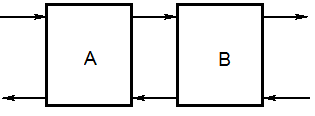
\includegraphics[scale=0.5]{pictures/chainrepresentation.png}
	\caption{\texttt{chain(A:B)} puts blocks in sequence}
	\label{fig:chainrepresentation}
\end{figure}

This basic component \texttt{chain} comes along with termination components and excitation functions. The terminations are based on a generic \texttt{termination} operation (letting chains opened), which is specialized into \texttt{fullTerminations} (which closes chains), \texttt{leftTermination} and \texttt{rightTermination} (each closes only one end). Functions such as the Dirac impulse or a noise burst~\cite{lac_orlarey} have been developed to excite instruments.

\section{Physical modeling with \texttt{pm.lib}}

We describe some preliminary use cases for the \texttt{pm.lib} library.

\subsection*{Strings}

We are now equipped to build our first physical-modeling-based instrument: an ideal string. First, the \texttt{waveguide} model is written using a $4^{th}$-order fractional delay for each delay line with a \texttt{n}-sample length:\\
\\
\texttt{waveguide(nMax,n) = fdelay4(nMax,n),fdelay4(nMax,n),\_;}\\

An ideal string is then written as:\\
\\
\texttt{idealString(l,r, pluck,x) = fullTerminations(term,wg,term)\\
~~~~with \{...\};	
} \\

\noindent where we specify the string length \texttt{l}, the reflection coefficient (or filter) \texttt{r} and the pluck position \texttt{pluck} (in the interval 0-0.99); \texttt{wg} is the previous \texttt{waveguide} function and \texttt{term} is calculated with the given parameters, while \texttt{x} is the input of the system (excitation function).

This \texttt{idealString} function led to other functions like \texttt{steelString} and \texttt{nylonString} where the reflection coefficient of -1 has been replaced by a damping filter designed by ear to sound the most accurately as possible.


Those two scripts were written  for the same goal: to recreate the sound of an object when stricking by an small impulse. With a functional and powerful algorithm, it would be possible to model any object vibration sound which lead to many musically beautiful possibilities.

\subsection*{Percussion}

\texttt{IR2dsp.py} is a python script that aims to recreate the sound of a stricking object, giving its impulse response (IR) in input. It outputs a filterbank model of the object written in a Faust \texttt{dsp} file.

The algorithm is divided into several steps. First, a Fourier Fast Transform (FFT) computes the power spectrum of the IR. Then, we detect the frequency peaks in the data provided by the FFT, with information from the input parameters such as minimum frequency threshold and minimum peak distance. The algorithm then analyzes each detected peak to compute the width of each one.

Finally, the script has been able to compute three parameters to describe each peak: the central frequency, the value of the peak (the gain in dB) and the width, which is transformed into audio decay time\footnote{ccrma.stanford.edu/\~{}jos/mdft/Audio\_Decay\_Time\_T60}. Each triplet of parameters describes a bandpass filter of the shape of the corresponding peak. Finally, put together, this yields a filterbank of bandpass filters (see Figure~\ref{fig:filterbank}) that recreates with some accuracy the sound of the corresponding object when excited.

\begin{figure}[h]
	\centering
	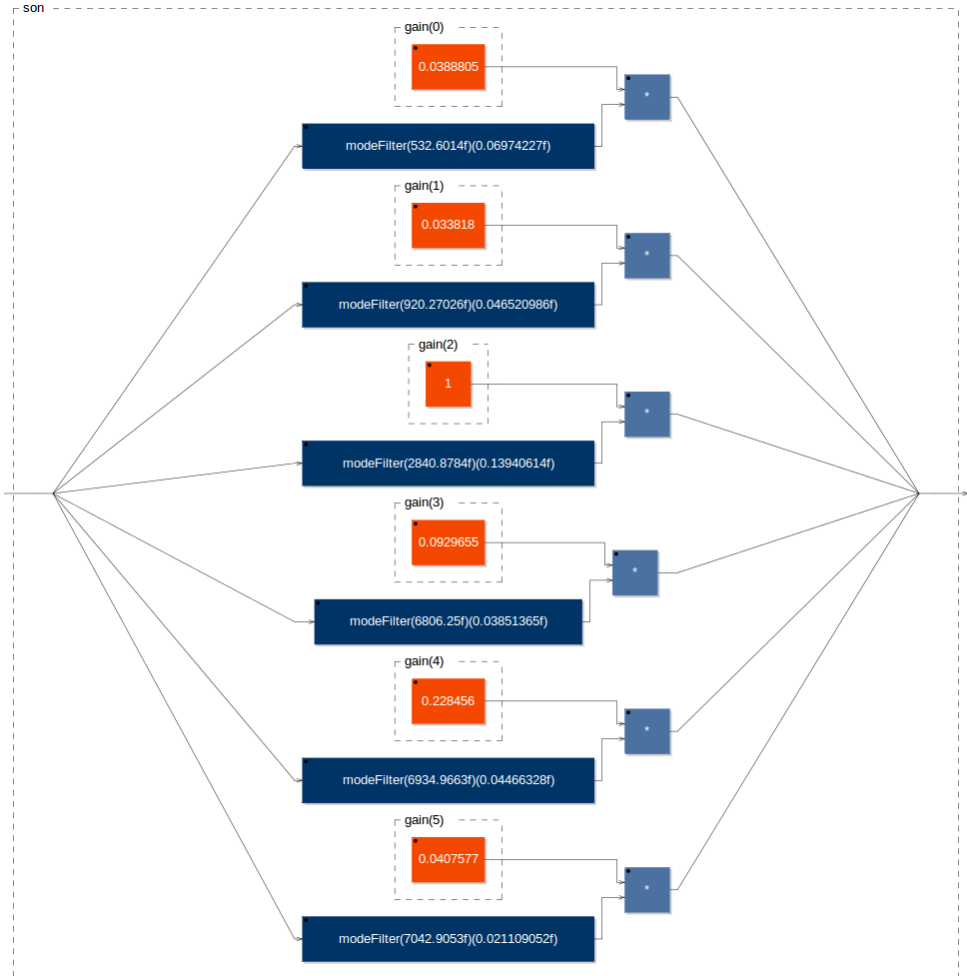
\includegraphics[scale=0.2]{pictures/filterbankdiagram.png}
	\caption{Filterbank from the IR of a glass}
	\label{fig:filterbank}
\end{figure}

\subsection*{Generic object}

A second script, \texttt{mesh2dsp.py}, aims to generate the same result, i.e., the creation of a filterbank model written in Faust, but here to recreate the sound of any vibrating object. Given a geometric file (\texttt{.stl} file) specifying the shape of an object, the script performs a Finite Element Analysis (FEA) via the open-source software Elmer\footnote{https://www.csc.fi/web/elmer}. Three parameters have to be given for the FEA as inputs of the script: the Young modulus, the Poisson coefficient and the density of the material of the object.

The algorithm extracts from the FEA output the computed eigenvalues that are transformed then into frequencies. With those frequencies, we are able to generate the previously explained filterbank model, except that we are missing two parameters: the power of each filter (gain in dB) and the audio decay time. The audio decay time cannot be computed from a FEA. The gain of each vibration frequencies can be retrieved from the FEA, and we intend to do so in future work. 
A difficulty of this method is that, during the FEA, one needs to specify some immobility constraints (e.g., both ends of a string), which makes the algorithm less automated.

\section{Conclusion}

We presented the work that has been begun on a physical modeling library in the Faust audio language. We gave a quick tour of what physical modeling synthesis is, and then a quick review of the manner one can write audio programs in Faust. We introduced the need for a physical modeling library by pointing out that Faust is not fully operational for physical modeling in its present form, and then the application of the library was illustrated with somet sounding pieces of instrument. We finally presented two scripts, the goal of which is very promising, even with some limitations, especially with the FEA.

Future works will focus on proposing more instrument elements to provide a modular audio library to construct instruments piece by piece. The first presented python script works well, but the second one needs future work.

\section{Acknowledgements}

Our thanks go to Yann Orlarey for his help with the use of Faust.

\bibliographystyle{acl}
\bibliography{sample}

\end{document}
